\chapter{Planes Detection}

Not all changes are relevant for analysis in the context of construction sites. The main objects to compare would be the core structure of a building while humans and construction tools can be disregarded as noise.\\

Since buildings contain many planar structures like walls and ceilings, one can take advantage of this simple geometry to extract flat surfaces from the point cloud data. This approach provides a primitive noise filtering and a planar segmentation which allows the ability to later compare planes together.\\

This chapter explores multiple popular methods that are relevant for plane detection in point clouds, namely Generalised Hough Transform and RANSAC. Those algorithms will be described and improvements made to these algorithms will be discussed to provide a comprehensive overview of planes detection techniques.

\section{Generalised Hough Transform}

The Generalised Hough Transform is a classical feature detection technique in computer vision and digital image processing that was initially used to identify lines, circles, and ellipses in 2D images \cite{hough1962}. But it has since been extended to a wide range of applications such as plane detection in point cloud \cite{hough3d}.\\

\noindent The method can be decomposed in three steps:
\begin{enumerate}
    \item Given an input point cloud, the algorithm maps each data point of the original space to a discretized parameter space representation. This parameter space is judiciously selected to fit models such as plane equations.
    \item Then, the algorithm systematically explores all possible plane equations within the parameter space. For each of those candidate plane equations, a voting process is conducted and the results are cast in an accumulator.
    \item Based on the accumulator, the algorithm selects the most probable planes which are planes with a higher number of votes.
\end{enumerate}
\begin{figure}[ht]
    \centering
    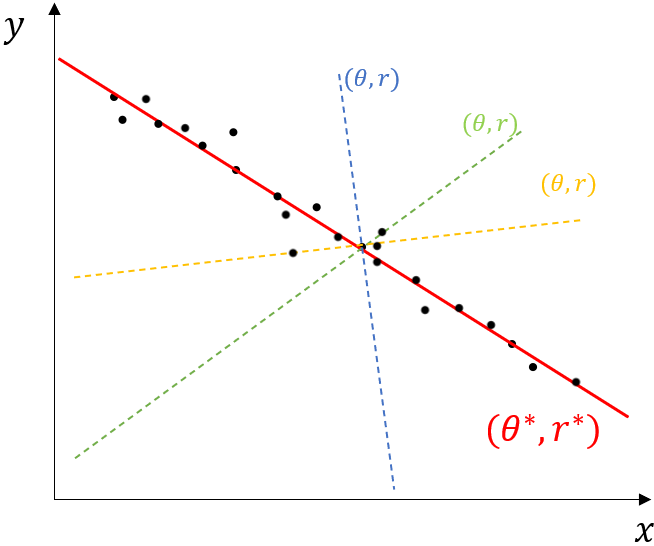
\includegraphics[scale=0.8]{Img/03_GHT.png}
    \caption{Illustration of the Generalised Hough Transform for line detection. Each one of those lines is described by parameters $(\theta,r)$. The best line $(\theta, r)$, illustrated in red, is the one with the most inliers.}
\end{figure}
More specifically, a plane in the original space is given by a normal vector $n = (n_x,n_y,n_z)$ and a distance to the origin $r$. All point $p = (p_x, p_y, p_z) $ which belong to the plane fit the following equation:
\begin{equation}
    p_x n_x + p_y n_y + p_z n_z = r
\end{equation}
Moreover, a plane can be described in a spherical coordinate $(r, \theta,\phi)$ which will be the parameter space (Eq \ref{eq:HT_polar}). Given this space, the algorithm will discretize the space and perform a voting process.
\begin{equation}
    p_x \cos(\theta) \sin(\phi) + p_y \sin(\theta)\sin(\phi) + z \cos(\phi) = r
    \label{eq:HT_polar}
\end{equation}

\begin{algorithm}[ht]
\caption{Generalised Hough Transform (GHT)}\label{alg:HT}
\begin{description}[leftmargin=!, labelwidth=\widthof{\textbf{Step1: }}]
    \item [Step 1] Let $(r_i, \theta_j, \phi_k)$ be cells of the discretized parameter space. Let $x_m$ be a point in the given point cloud $X$, and $A$ be the accumulator. 
    \item [Step 2] For each cells $(r_i, \theta_j, \phi_k)$, find the number of points $x_m$ that lies on the plane, denoted as $n_{ijk}$, with the equation  \ref{eq:HT_polar}. And update the accumulator:
        \[
            A[i,j,k] = n_{ijk}
        \]
    \item [Step 3] Search the cell with the local maximal score.
\end{description}
\end{algorithm}


One of the major drawbacks of the GHT is its long computation time. Specifically, the second step of the Algorithm \ref{alg:HT}, which involves incrementing the cells of the accumulator, requires a computational complexity of $\mathcal{O}(|X| \cdot N_\theta \cdot N_\phi)$. Consequently, researchers have conducted studies to enhance its efficiency \cite{hough3d}.\\

The first approach to address this issue is known as the Probabilistic Hough Transform (PHT). This method aims to decrease the number of points involved during this second step by selecting randomly a few of them reducing the computational complexity \cite{probaHT}.\\

Another technique employed is the Adaptive Probabilistic Hough Transform (APHT) which adds a stopping criterion by monitoring the accumulator. Once a stable structure emerges, the algorithm terminates, thereby avoiding unnecessary computations and further reducing the overall processing time \cite{adaptiveprobaHT}.

\section{RANSAC for plane detection}
RANSAC is also a popular stochastic method used for plane detection due to its robustness against outliers and its simplicity.\\

As discussed in the previous chapter on global registration, this method follows a similar approach by selecting random points in a point cloud to fit a model. Then it evaluates the number of inliers that fit a candidate model and returns a consensus  based on the agreement among the majority of the data samples.\\

In the specific case of plane detection in a point cloud, the RANSAC algorithm (Algorithm \ref{alg:RANSAC_Plane}) chooses 3 points $x_1,x_2,x_3$ and utilizes them to fit a plane. Afterward, it identifies inliers and outliers point from the initial point cloud and returns the plane that possesses the largest amount of inliers \cite{ransac_planedetection}.
\begin{figure}[ht]
    \centering
    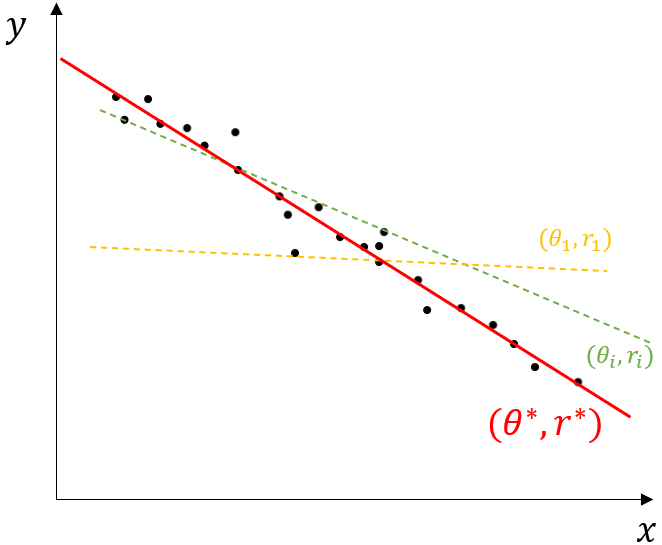
\includegraphics[scale=0.8]{Img/03_RANSAC2.png}
    \caption{Illustration RANSAC algorithm for line detection. The algorithm selects 2 random points to define a line. The one with the best number of inliers, depicted in red, is considered the best fit.}
    \label{fig:ransac_illustration}
\end{figure}

\begin{algorithm}[ht]
\caption{RANSAC (Plane Detection)}\label{alg:RANSAC_Plane}
\begin{description}[leftmargin=!, labelwidth=\widthof{\textbf{Step1: }}]
    \item [Step 1:] Let $X$ be the source point cloud. We denote $x$ as a point of $X$ and $n_x$ as the estimated normal for this point.
    \item [Step 2:] Select a random subset of 3 points $ x_1,x_2,x_3\subset X$ which describe a candidate plane $P$
    \item [Step 3:] Compute the vectors 
        \[\vec{u} = x_2 - x_1 \; \; \; \; \; \vec{v} = x_3 - x_1\]
    \item [Step 4:] Compute the plane normal 
        \[\vec{n} = \frac{\vec{u} \times \vec{v} }{\| \vec{u} \times \vec{v}\| }\]
    \item [Step 5:] For all $x \in X \backslash X'$, determine if it is an inlier or an outlier based on the following criterion:
    \[ \text{dist}(P,x) \leq trsh_d \; \; \; \; \; n_x \cdot \vec{n} \geq trsh_n\]
    \item [Step 6:] Repeat \textbf{Step2 - Step5} a pre-determined number of time $k$. Return the candidate plane $P$ with the largest amount of inliers.
\end{description}
\end{algorithm}

\begin{figure}[ht]
    \centering
    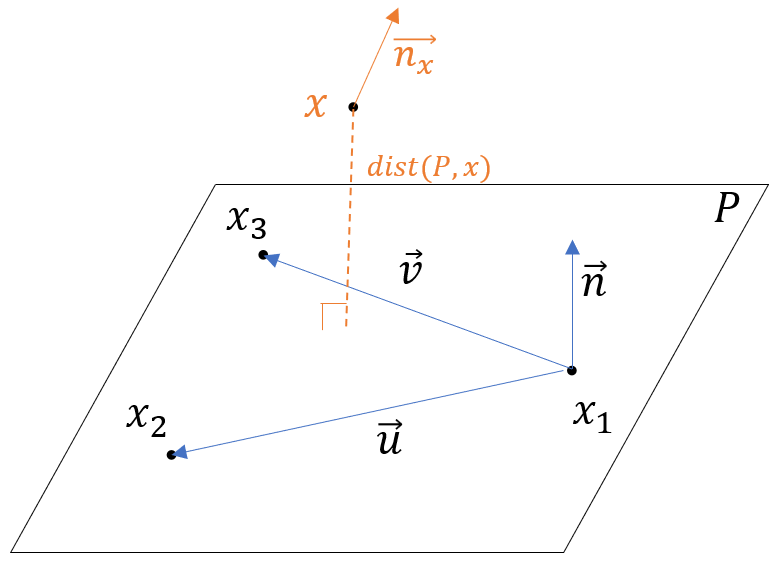
\includegraphics[scale=0.4]{Img/03_RANSAC.png}
    \caption{Illustration of the symbols described in Algorithm \ref{alg:RANSAC_Plane}}
    \label{fig:ght_illustration}
\end{figure}
The number of iteration $k$ performed by the algorithm can be expressed in function of the desired probability success. If we define $w$ as the probability of choosing one inlier in the dataset as in Equation \ref{eq:proba_1inlier}, the probability of choosing 3 inliers becomes $w^3$.
\begin{equation}\label{eq:proba_1inlier}
    w = \frac{\text{number of inliers}}{\text{number of points}}
\end{equation}
 The probability that the algorithm never selects 3 inliers after $k$ iteration, denoted as $(1-p)$, becomes:
 \begin{equation}
     (1-p) = (1-w^3)^k
 \end{equation}
 And thus, the number of iteration can be parametrized in the function of the confidence probability $p$ as follow:
 \begin{equation}
     k = \frac{\log (1-p)}{\log (1- w^n)}
 \end{equation}

The parameters $trsh_d$ and $trsh_n$ in the criterion in \textbf{Step 5} can be chosen wisely depending on the accuracy and noise of the point cloud measurement and normal estimates.\\

The RANSAC algorithm (Algorithm \ref{alg:RANSAC_Plane}), unlike the Generalised Hough Transform (Algorithm \ref{alg:HT}), extracts one plane at a time. Hence, the algorithm needs to be recursively used to extract all planes in a point cloud. Each time, we remove the points belonging to the plane at a given iteration.
